%!TEX root = ../Final_Assignment_SP_ML4IM_2023.tex
\chapter{Discussion}
\label{ch:discussion}

% mittel ausführlich
% alle

As seen in chapter \ref{ch:results}, the results of the project are extremly bad, so much that there is no point in using the resulting models for any kind of further research. But the results are so bad, that for one it is unlikly that these results are representative, which means that some problems must have accured during the workflow, as well as that it is worth discussing why the results are so bad, what may have happend and what could be done to improve them. \\
Because these circumstaces this chapter will not discuss the results further, but will deal with the problems that may have caused these results.

The first point to examine would be the preprocessing of the data. There are multiple problems that could arise in this step. The most prominent would be, that the prepocessing of the videos would lead to unusable or corrupt videos files. But as shown in chapter \ref{ch:methods} the outputs are correct. Some preprocessing steps provide visually better outputs to classify insect, like the background subtraction compared to the HSV, but all results servicable to yield some results. \\
Another problem could be, that the preprocessing of the images lead to a shift in the time steps of the videos.

This leads to the bounding boxes, as a shift in the time steps could lead to issues with mapping the bounding boxes correctly. 
\begin{figure}[h]
    \centering
    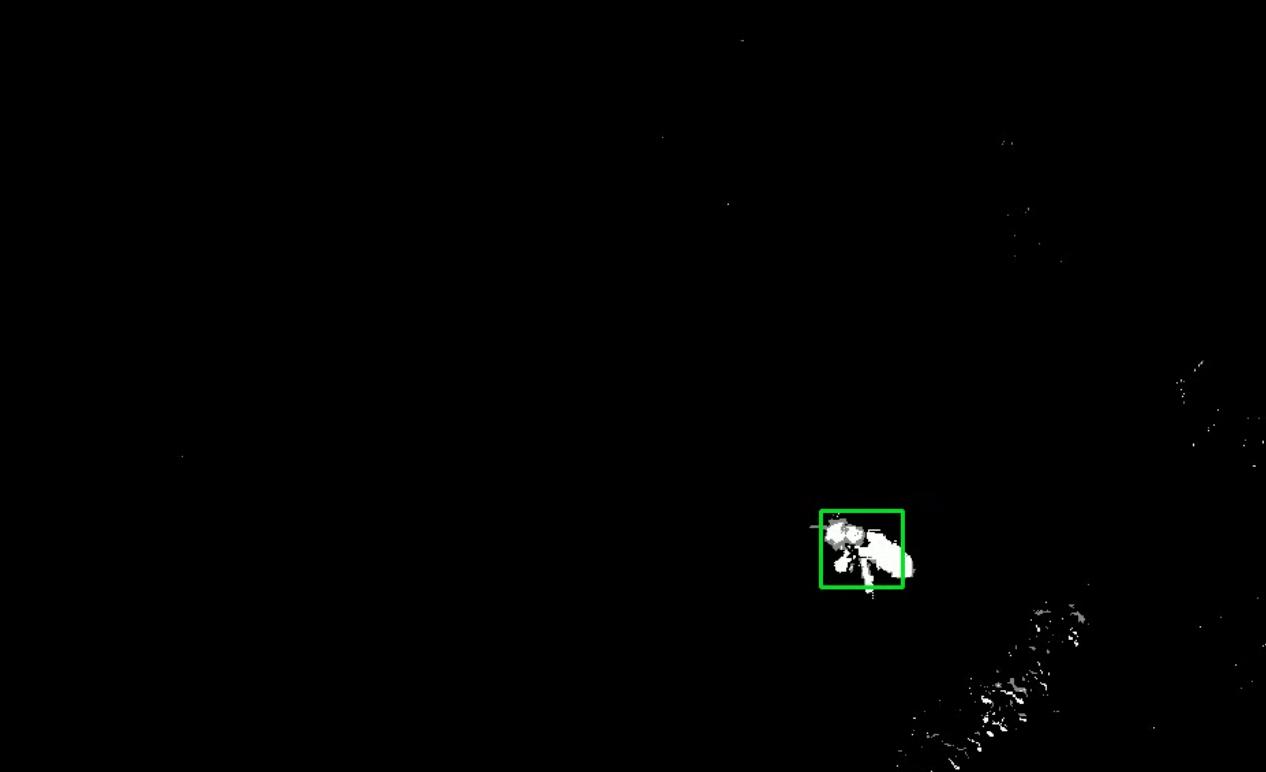
\includegraphics[width=0.5\textwidth]{images/bb_test_backSub.png}
    \caption{Combination of the preprocessed video using background subtraction and the corresponding bounding boxes}
\end{figure}

\begin{figure}[h]
    \centering
    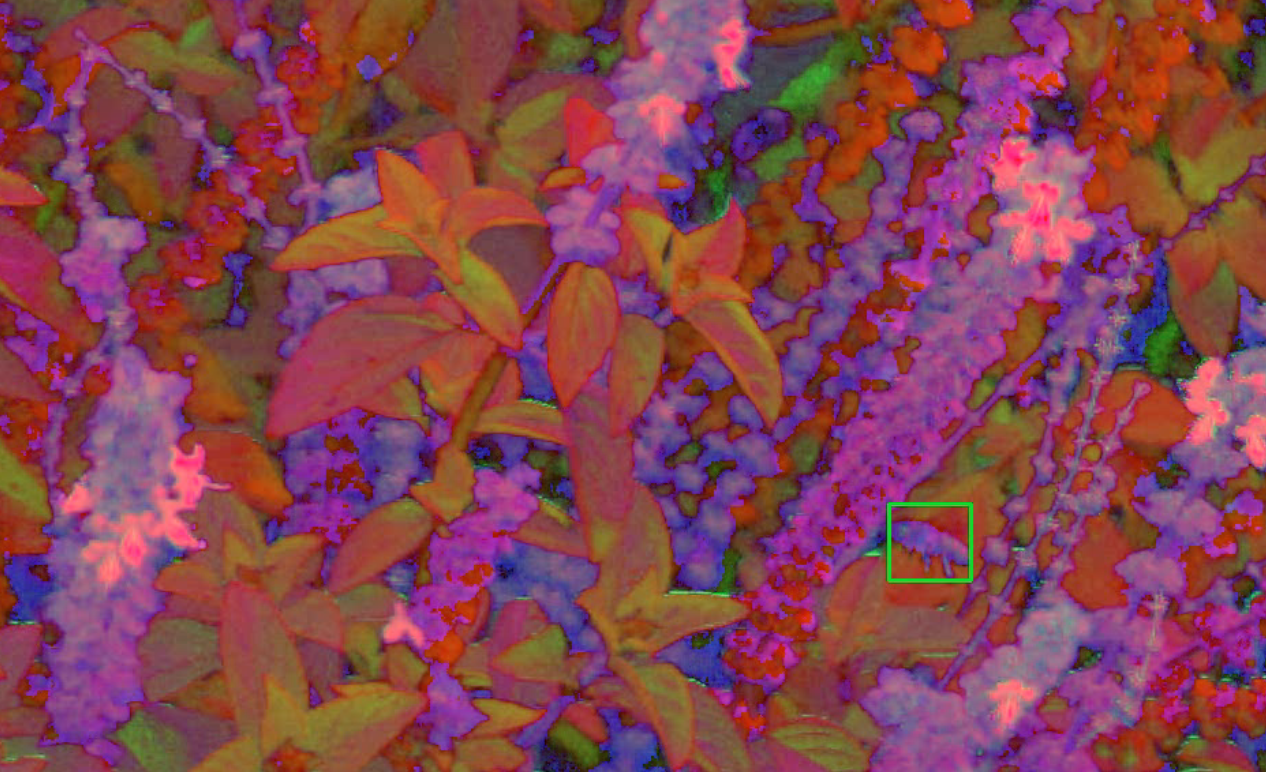
\includegraphics[width=0.5\textwidth]{images/bb_test_HSV.png}
    \caption{Combination of the preprocessed video using RGB to HSV and the corresponding bounding boxes}
\end{figure}
But as shown in the pictures above, the bounding boxes are correctly mapped to the videos. \\
As visible in the pictures the bounding boxes are not perfect and could be improved, but they are good enought to be used for training a model. The improvement of the bounding boxes could lead to minimal better results if you want to improve a already good model, but in this case the bounding boxes are not the problem.

As these points are not the problem, the next point to examine would be the training of the model. \\
As shown in chapter \ref{ch:methods} the training of the model was done using the YOLOv8 model. A possibility here could be that the default YOLOv8 model is not suitable to identify insects in the RGB or our preprocessed videos. But considering the results of the study shown in chapter \ref{ch:related_work}, which used YOLO to identify and classify street signs in RGB videos with results up to 83.2\% in the mAP@0.5 score, it is safe to assume that the YOLOv8 model should be suitable for this task. 

All the above mentioned points were problems and approaches we checked and made sure that these are not the root of the problems. The next paragraphs will discuss some other points that could have impacted the results of the models.

% Hier müssen jetzt noch die punkt eingefügt werden (siehe unten)


% \begin{itemize}
%     \item RGB ist nicht ausreichend
%     \item Crossvalidation wäre noch eine Möglichkeit
%     \item zu wenig Trainingsdaten; schlechte Datenqualität
%     \item mal Hyperparameter untersuchen
% \end{itemize}

